\documentclass[tikz]{standalone}
\usepackage[utf8]{inputenc}

\begin{document}

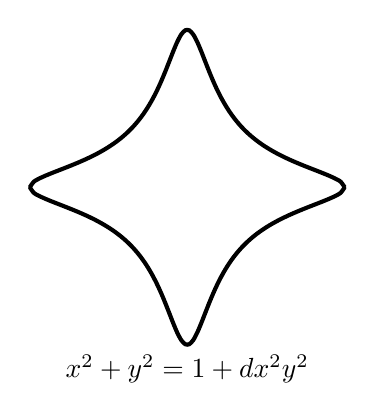
\begin{tikzpicture}[scale=2]
\path[smooth,samples=80,line width=1.5pt,draw] plot[domain=-1:1] (\x, {sqrt((1 - (\x)^2)/(1 + 42*(\x)^2))}) plot[domain=1:-1] (\x, {-sqrt((1 - (\x)^2)/(1 + 42*(\x)^2))});
\fill (1,0) circle (.3pt);
\fill (-1,0) circle (.3pt);
\node[below] at (0,-1) {$x^2 + y^2 = 1 + dx^2y^2$};
\end{tikzpicture}

\end{document}